\cajita{Población de 15 años o más por sector económico, según sexo }{El sector informal guatemalteco comprende a la Población Ocupada (PO) que labora como empleadores, empleados y obreros de empresas con menos de 6 personas, trabajadores por cuenta propia o autónoma (excluyendo profesionales y técnicos), familiares no remunerados de los empleadores o personas ocupadas en servicio doméstico. Su contraparte, el sector formal, está comprendido por la población ocupada que no está en el sector informal. 

En el año 2022 las mujeres integraron el 27.9\% del sector informal y el 9.2\% del sector formal. }{Población de 15 años o más por sector económico, según sexo}{República de Guatemala, Instituto Nacional de Estadística -INE-, en porcentaje}{\begin{tikzpicture}[x=1pt,y=1pt]% Created by tikzDevice version 0.12.4 on 2023-05-04 15:41:55
% !TEX encoding = UTF-8 Unicode
\definecolor{fillColor}{RGB}{255,255,255}
\path[use as bounding box,fill=fillColor,fill opacity=0.00] (0,0) rectangle (289.08,198.74);
\begin{scope}
\path[clip] (  0.00,  0.00) rectangle (289.08,198.74);

\path[] (  0.00,  0.00) rectangle (289.08,198.74);
\end{scope}
\begin{scope}
\path[clip] (  0.00,  0.00) rectangle (289.08,198.74);
\definecolor{fillColor}{RGB}{54,50,131}

\path[fill=fillColor] ( 23.00, 21.09) rectangle ( 75.55, 52.92);

\path[fill=fillColor] (154.39, 21.09) rectangle (206.95,117.47);
\definecolor{fillColor}{RGB}{116,112,200}

\path[fill=fillColor] ( 82.13, 21.09) rectangle (134.68, 89.08);

\path[fill=fillColor] (213.53, 21.09) rectangle (266.08,170.58);
\definecolor{drawColor}{RGB}{0,0,0}

\path[draw=drawColor,line width= 0.6pt,line join=round] (-289.08, 21.09) -- (578.16, 21.09);

\node[text=drawColor,anchor=base,inner sep=0pt, outer sep=0pt, scale=  0.83] at ( 49.27, 56.15) {9.2};

\node[text=drawColor,anchor=base,inner sep=0pt, outer sep=0pt, scale=  0.83] at (180.68,120.70) {27.9};

\node[text=drawColor,anchor=base,inner sep=0pt, outer sep=0pt, scale=  0.83] at (108.41, 92.31) {19.7};

\node[text=drawColor,anchor=base,inner sep=0pt, outer sep=0pt, scale=  0.83] at (239.81,173.81) {43.2};

\path[] (  0.00, 21.09) rectangle (289.08,170.58);

\path[] ( 78.84, 21.09) --
	( 78.84,170.58);

\path[] (210.24, 21.09) --
	(210.24,170.58);

\path[] (  0.00, 21.09) rectangle (289.08,170.58);
\end{scope}
\begin{scope}
\path[clip] (  0.00,  0.00) rectangle (289.08,198.74);

\path[] (  0.00, 21.09) --
	(  0.00,170.58);
\end{scope}
\begin{scope}
\path[clip] (  0.00,  0.00) rectangle (289.08,198.74);

\path[] (  0.00, 21.09) --
	(289.08, 21.09);
\end{scope}
\begin{scope}
\path[clip] (  0.00,  0.00) rectangle (289.08,198.74);

\path[] ( 78.84, 18.34) --
	( 78.84, 21.09);

\path[] (210.24, 18.34) --
	(210.24, 21.09);
\end{scope}
\begin{scope}
\path[clip] (  0.00,  0.00) rectangle (289.08,198.74);
\definecolor{drawColor}{RGB}{0,0,0}

\node[text=drawColor,anchor=base,inner sep=0pt, outer sep=0pt, scale=  1.00] at ( 78.84,  7.01) {Formal};

\node[text=drawColor,anchor=base,inner sep=0pt, outer sep=0pt, scale=  1.00] at (210.24,  7.01) {infromal};
\end{scope}
\begin{scope}
\path[clip] (  0.00,  0.00) rectangle (289.08,198.74);
\coordinate (apoyo) at (59.42,189.21);
\coordinate (longitudFicticia) at (7.11,9.53);
\coordinate (longitud) at (7.11,7.11);
\coordinate (desX) at (135.34,0);
\coordinate (desY) at (0,1.21);
\definecolor[named]{ct1}{HTML}{
363283
}
\definecolor[named]{ct2}{HTML}{
7470C8
}
\definecolor[named]{ctb1}{HTML}{
363283
}
\definecolor[named]{ctb2}{HTML}{
7470C8
}
\path [fill=none] (apoyo) rectangle ($(apoyo)+(longitudFicticia)$)
node [xshift=0.3cm,inner sep=0pt, outer sep=0pt,midway,right,scale = 0.9]{Mujer};
\draw [color = ctb1,fill=ct1] ( $(apoyo)  + (desY) $) rectangle ($(apoyo)+ (desY) +(longitud)$);
\path [fill=none] ($(apoyo)+(desX)$) rectangle ($(apoyo)+(desX)+(longitudFicticia)$)
node [xshift=0.3cm,inner sep=0pt, outer sep=0pt,midway,right,scale = 0.9]{Hombre};
\draw [color = ctb2 ,fill=ct2] ( $(apoyo)  + (desY) + (desX) $) rectangle ($(apoyo)+ (desY)+ (desX) +(longitud)$);
\end{scope}
\end{tikzpicture}}{INE - ENEI 2022}{}

\cajita{Tasa de participación económica por dominio de estudio, sexo y estado conyugal}{Se definio el estado conyugal "con pareja" a personas que reportaron estar casadas y unidas y "sin pareja" a personas que reportaron estar solteras, divorciadas, viudas o separadas.  

Para 2022, en la PEA las mujeres "sin pareja" en el dominio Urbano Metropolitano representaron el 4.9\% y "con pareja" el 3.7\%. En el Resto Urbano aquellas mujeres "sin pareja" reportaron el 5.4\% de participación en la PEA y mujeres "con pareja" reportaron 5.3\% de participación. En el dominio Rural Nacional la participación de mujeres "con pareja" y "sin pareja" en la PEA que fue del 9.2\%. 
}{Tasa de participación económica por dominio de estudio, sexo y estado conyougal}{República de Guatemala, Instituto Nacional de Estadística -INE- en porcentaje} {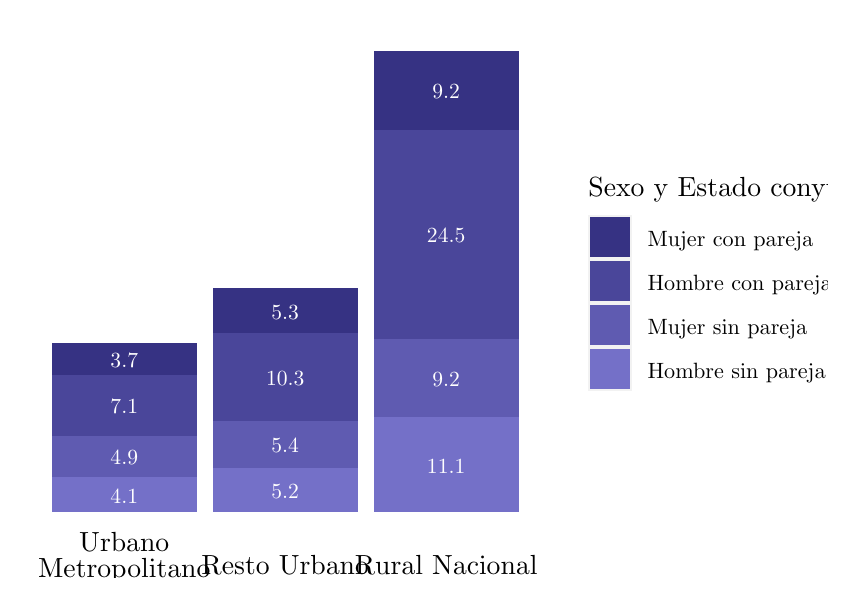
\begin{tikzpicture}[x=1pt,y=1pt]% Created by tikzDevice version 0.12.4 on 2023-04-26 12:29:30
% !TEX encoding = UTF-8 Unicode
\definecolor{fillColor}{RGB}{255,255,255}
\path[use as bounding box,fill=fillColor,fill opacity=0.00] (0,0) rectangle (289.08,198.74);
\begin{scope}
\path[clip] (  0.00,  0.00) rectangle (289.08,198.74);

\path[] (  0.00,  0.00) rectangle (289.08,198.74);
\end{scope}
\begin{scope}
\path[clip] (  0.00,  0.00) rectangle (289.08,198.74);
\definecolor{fillColor}{RGB}{54,50,131}

\path[fill=fillColor] (  8.72, 73.17) rectangle ( 61.07, 84.70);
\definecolor{fillColor}{RGB}{74,70,154}

\path[fill=fillColor] (  8.72, 51.27) rectangle ( 61.07, 73.17);
\definecolor{fillColor}{RGB}{95,91,177}

\path[fill=fillColor] (  8.72, 36.28) rectangle ( 61.07, 51.27);
\definecolor{fillColor}{RGB}{116,112,200}

\path[fill=fillColor] (  8.72, 23.73) rectangle ( 61.07, 36.28);
\definecolor{fillColor}{RGB}{54,50,131}

\path[fill=fillColor] ( 66.89, 88.38) rectangle (119.23,104.62);
\definecolor{fillColor}{RGB}{74,70,154}

\path[fill=fillColor] ( 66.89, 56.55) rectangle (119.23, 88.38);
\definecolor{fillColor}{RGB}{95,91,177}

\path[fill=fillColor] ( 66.89, 39.80) rectangle (119.23, 56.55);
\definecolor{fillColor}{RGB}{116,112,200}

\path[fill=fillColor] ( 66.89, 23.73) rectangle (119.23, 39.80);
\definecolor{fillColor}{RGB}{54,50,131}

\path[fill=fillColor] (125.05,161.89) rectangle (177.39,190.41);
\definecolor{fillColor}{RGB}{74,70,154}

\path[fill=fillColor] (125.05, 86.22) rectangle (177.39,161.89);
\definecolor{fillColor}{RGB}{95,91,177}

\path[fill=fillColor] (125.05, 57.97) rectangle (177.39, 86.22);
\definecolor{fillColor}{RGB}{116,112,200}

\path[fill=fillColor] (125.05, 23.73) rectangle (177.39, 57.97);
\definecolor{drawColor}{RGB}{255,255,255}

\node[text=drawColor,anchor=base,inner sep=0pt, outer sep=0pt, scale=  0.78] at ( 34.90, 75.90) {3.7};

\node[text=drawColor,anchor=base,inner sep=0pt, outer sep=0pt, scale=  0.78] at ( 34.90, 59.18) {7.1};

\node[text=drawColor,anchor=base,inner sep=0pt, outer sep=0pt, scale=  0.78] at ( 34.90, 40.74) {4.9};

\node[text=drawColor,anchor=base,inner sep=0pt, outer sep=0pt, scale=  0.78] at ( 34.90, 26.97) {4.1};

\node[text=drawColor,anchor=base,inner sep=0pt, outer sep=0pt, scale=  0.78] at ( 93.06, 93.47) {5.3};

\node[text=drawColor,anchor=base,inner sep=0pt, outer sep=0pt, scale=  0.78] at ( 93.06, 69.43) {10.3};

\node[text=drawColor,anchor=base,inner sep=0pt, outer sep=0pt, scale=  0.78] at ( 93.06, 45.14) {5.4};

\node[text=drawColor,anchor=base,inner sep=0pt, outer sep=0pt, scale=  0.78] at ( 93.06, 28.73) {5.2};

\node[text=drawColor,anchor=base,inner sep=0pt, outer sep=0pt, scale=  0.78] at (151.22,173.12) {9.2};

\node[text=drawColor,anchor=base,inner sep=0pt, outer sep=0pt, scale=  0.78] at (151.22,121.02) {24.5};

\node[text=drawColor,anchor=base,inner sep=0pt, outer sep=0pt, scale=  0.78] at (151.22, 69.06) {9.2};

\node[text=drawColor,anchor=base,inner sep=0pt, outer sep=0pt, scale=  0.78] at (151.22, 37.82) {11.1};

\path[] (  0.00, 15.40) rectangle (186.12,198.74);
\end{scope}
\begin{scope}
\path[clip] (  0.00,  0.00) rectangle (289.08,198.74);

\path[] (  0.00, 15.40) --
	(  0.00,198.74);
\end{scope}
\begin{scope}
\path[clip] (  0.00,  0.00) rectangle (289.08,198.74);

\path[] (  0.00, 15.40) --
	(186.12, 15.40);
\end{scope}
\begin{scope}
\path[clip] (  0.00,  0.00) rectangle (289.08,198.74);

\path[] ( 34.90, 12.65) --
	( 34.90, 15.40);

\path[] ( 93.06, 12.65) --
	( 93.06, 15.40);

\path[] (151.22, 12.65) --
	(151.22, 15.40);
\end{scope}
\begin{scope}
\path[clip] (  0.00,  0.00) rectangle (289.08,198.74);
\definecolor{drawColor}{RGB}{0,0,0}

\node[text=drawColor,anchor=base,inner sep=0pt, outer sep=0pt, scale=  1.00] at ( 34.90,  9.32) {Urbano};

\node[text=drawColor,anchor=base,inner sep=0pt, outer sep=0pt, scale=  1.00] at ( 34.90,  0.00) {Metropolitano};

\node[text=drawColor,anchor=base,inner sep=0pt, outer sep=0pt, scale=  1.00] at ( 93.06,  1.32) {Resto Urbano};

\node[text=drawColor,anchor=base,inner sep=0pt, outer sep=0pt, scale=  1.00] at (151.22,  1.32) {Rural Nacional};
\end{scope}
\begin{scope}
\path[clip] (  0.00,  0.00) rectangle (289.08,198.74);
\definecolor{fillColor}{RGB}{255,255,255}

\path[fill=fillColor] (197.12, 61.80) rectangle (289.08,152.34);
\end{scope}
\begin{scope}
\path[clip] (  0.00,  0.00) rectangle (289.08,198.74);
\definecolor{drawColor}{RGB}{0,0,0}

\node[text=drawColor,anchor=base west,inner sep=0pt, outer sep=0pt, scale=  1.00] at (202.62,137.71) {Sexo y Estado conyugal};
\end{scope}
\begin{scope}
\path[clip] (  0.00,  0.00) rectangle (289.08,198.74);
\definecolor{fillColor}{gray}{0.95}

\path[fill=fillColor] (202.62,115.00) rectangle (218.51,130.90);
\end{scope}
\begin{scope}
\path[clip] (  0.00,  0.00) rectangle (289.08,198.74);
\definecolor{fillColor}{RGB}{54,50,131}

\path[fill=fillColor] (203.33,115.71) rectangle (217.80,130.18);
\end{scope}
\begin{scope}
\path[clip] (  0.00,  0.00) rectangle (289.08,198.74);
\definecolor{fillColor}{gray}{0.95}

\path[fill=fillColor] (202.62, 99.10) rectangle (218.51,115.00);
\end{scope}
\begin{scope}
\path[clip] (  0.00,  0.00) rectangle (289.08,198.74);
\definecolor{fillColor}{RGB}{74,70,154}

\path[fill=fillColor] (203.33, 99.81) rectangle (217.80,114.28);
\end{scope}
\begin{scope}
\path[clip] (  0.00,  0.00) rectangle (289.08,198.74);
\definecolor{fillColor}{gray}{0.95}

\path[fill=fillColor] (202.62, 83.20) rectangle (218.51, 99.10);
\end{scope}
\begin{scope}
\path[clip] (  0.00,  0.00) rectangle (289.08,198.74);
\definecolor{fillColor}{RGB}{95,91,177}

\path[fill=fillColor] (203.33, 83.91) rectangle (217.80, 98.38);
\end{scope}
\begin{scope}
\path[clip] (  0.00,  0.00) rectangle (289.08,198.74);
\definecolor{fillColor}{gray}{0.95}

\path[fill=fillColor] (202.62, 67.30) rectangle (218.51, 83.20);
\end{scope}
\begin{scope}
\path[clip] (  0.00,  0.00) rectangle (289.08,198.74);
\definecolor{fillColor}{RGB}{116,112,200}

\path[fill=fillColor] (203.33, 68.01) rectangle (217.80, 82.49);
\end{scope}
\begin{scope}
\path[clip] (  0.00,  0.00) rectangle (289.08,198.74);
\definecolor{drawColor}{RGB}{0,0,0}

\node[text=drawColor,anchor=base west,inner sep=0pt, outer sep=0pt, scale=  0.80] at (224.01,119.82) {Mujer con pareja};
\end{scope}
\begin{scope}
\path[clip] (  0.00,  0.00) rectangle (289.08,198.74);
\definecolor{drawColor}{RGB}{0,0,0}

\node[text=drawColor,anchor=base west,inner sep=0pt, outer sep=0pt, scale=  0.80] at (224.01,103.92) {Hombre con pareja};
\end{scope}
\begin{scope}
\path[clip] (  0.00,  0.00) rectangle (289.08,198.74);
\definecolor{drawColor}{RGB}{0,0,0}

\node[text=drawColor,anchor=base west,inner sep=0pt, outer sep=0pt, scale=  0.80] at (224.01, 88.02) {Mujer sin pareja};
\end{scope}
\begin{scope}
\path[clip] (  0.00,  0.00) rectangle (289.08,198.74);
\definecolor{drawColor}{RGB}{0,0,0}

\node[text=drawColor,anchor=base west,inner sep=0pt, outer sep=0pt, scale=  0.80] at (224.01, 72.12) {Hombre sin pareja};
\end{scope}
\end{tikzpicture}}{INE - ENEI 2022}{}

\cajita{PEA por sexo, según dominio de estudio (comparar 2018 y 2022)}{La población economicamente activa se integra por la polación en en edad de trabajar y la población ocupada. 

Para el 2022 las mujeres que integran PEA en el dominio urbano metropolitano aumento 0.9\%, en el resto urbano disminuyo 1.7\% y en el dominio rural aumento 4.5\%.}{PEA por sexo, según dominio de estudio (comparar 2018 y 2022}{República de Guatemala, Instituto Nacional de Estadística -INE- en porcentaje} {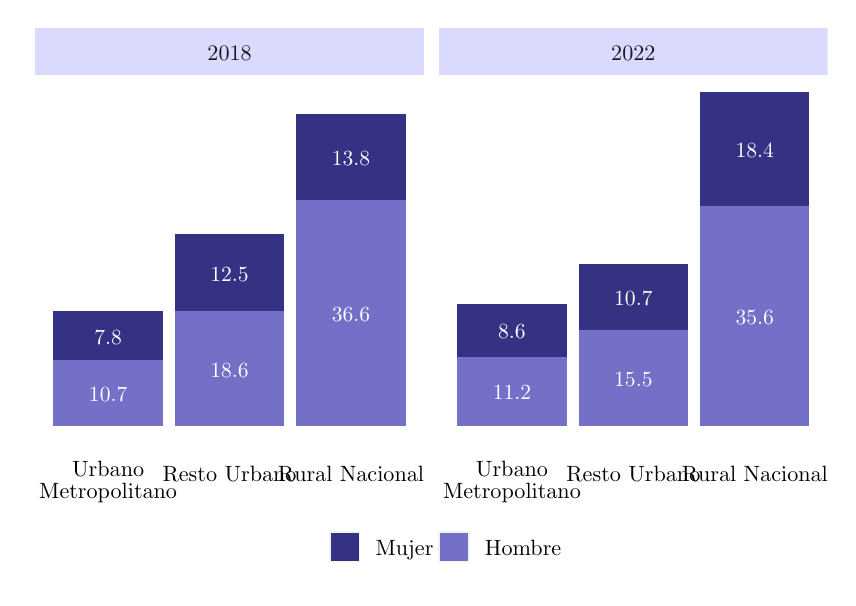
\begin{tikzpicture}[x=1pt,y=1pt]% Created by tikzDevice version 0.12.4 on 2023-05-04 16:27:01
% !TEX encoding = UTF-8 Unicode
\definecolor{fillColor}{RGB}{255,255,255}
\path[use as bounding box,fill=fillColor,fill opacity=0.00] (0,0) rectangle (289.08,198.74);
\begin{scope}
\path[clip] (  0.00,  0.00) rectangle (289.08,198.74);

\path[] (  0.00,  0.00) rectangle (289.08,198.74);
\end{scope}
\begin{scope}
\path[clip] (  0.00,  0.00) rectangle (289.08,198.74);
\definecolor{fillColor}{RGB}{54,50,131}

\path[fill=fillColor] (  9.33, 78.65) rectangle ( 48.82, 96.18);
\definecolor{fillColor}{RGB}{116,112,200}

\path[fill=fillColor] (  9.33, 54.82) rectangle ( 48.82, 78.65);
\definecolor{fillColor}{RGB}{54,50,131}

\path[fill=fillColor] ( 53.21, 96.27) rectangle ( 92.70,124.20);
\definecolor{fillColor}{RGB}{116,112,200}

\path[fill=fillColor] ( 53.21, 54.82) rectangle ( 92.70, 96.27);
\definecolor{fillColor}{RGB}{54,50,131}

\path[fill=fillColor] ( 97.09,136.64) rectangle (136.58,167.55);
\definecolor{fillColor}{RGB}{116,112,200}

\path[fill=fillColor] ( 97.09, 54.82) rectangle (136.58,136.64);
\definecolor{drawColor}{RGB}{255,255,255}

\node[text=drawColor,anchor=base,inner sep=0pt, outer sep=0pt, scale=  0.78] at ( 29.08, 84.39) {7.8};

\node[text=drawColor,anchor=base,inner sep=0pt, outer sep=0pt, scale=  0.78] at ( 29.08, 63.70) {10.7};

\node[text=drawColor,anchor=base,inner sep=0pt, outer sep=0pt, scale=  0.78] at ( 72.96,107.20) {12.5};

\node[text=drawColor,anchor=base,inner sep=0pt, outer sep=0pt, scale=  0.78] at ( 72.96, 72.51) {18.6};

\node[text=drawColor,anchor=base,inner sep=0pt, outer sep=0pt, scale=  0.78] at (116.84,149.06) {13.8};

\node[text=drawColor,anchor=base,inner sep=0pt, outer sep=0pt, scale=  0.78] at (116.84, 92.69) {36.6};

\path[] (  2.75, 54.82) --
	(143.16, 54.82);

\path[] (  2.75, 99.51) --
	(143.16, 99.51);

\path[] (  2.75,144.21) --
	(143.16,144.21);

\path[] (  2.75, 48.78) rectangle (143.16,181.58);
\end{scope}
\begin{scope}
\path[clip] (  0.00,  0.00) rectangle (289.08,198.74);
\definecolor{fillColor}{RGB}{54,50,131}

\path[fill=fillColor] (155.25, 79.76) rectangle (194.74, 98.98);
\definecolor{fillColor}{RGB}{116,112,200}

\path[fill=fillColor] (155.25, 54.82) rectangle (194.74, 79.76);
\definecolor{fillColor}{RGB}{54,50,131}

\path[fill=fillColor] (199.13, 89.52) rectangle (238.62,113.41);
\definecolor{fillColor}{RGB}{116,112,200}

\path[fill=fillColor] (199.13, 54.82) rectangle (238.62, 89.52);
\definecolor{fillColor}{RGB}{54,50,131}

\path[fill=fillColor] (243.01,134.43) rectangle (282.50,175.55);
\definecolor{fillColor}{RGB}{116,112,200}

\path[fill=fillColor] (243.01, 54.82) rectangle (282.50,134.43);
\definecolor{drawColor}{RGB}{255,255,255}

\node[text=drawColor,anchor=base,inner sep=0pt, outer sep=0pt, scale=  0.78] at (174.99, 86.34) {8.6};

\node[text=drawColor,anchor=base,inner sep=0pt, outer sep=0pt, scale=  0.78] at (174.99, 64.26) {11.2};

\node[text=drawColor,anchor=base,inner sep=0pt, outer sep=0pt, scale=  0.78] at (218.87, 98.43) {10.7};

\node[text=drawColor,anchor=base,inner sep=0pt, outer sep=0pt, scale=  0.78] at (218.87, 69.13) {15.5};

\node[text=drawColor,anchor=base,inner sep=0pt, outer sep=0pt, scale=  0.78] at (262.75,151.96) {18.4};

\node[text=drawColor,anchor=base,inner sep=0pt, outer sep=0pt, scale=  0.78] at (262.75, 91.59) {35.6};

\path[] (148.66, 54.82) --
	(289.08, 54.82);

\path[] (148.66, 99.51) --
	(289.08, 99.51);

\path[] (148.66,144.21) --
	(289.08,144.21);

\path[] (148.66, 48.78) rectangle (289.08,181.58);
\end{scope}
\begin{scope}
\path[clip] (  0.00,  0.00) rectangle (289.08,198.74);
\definecolor{fillColor}{RGB}{218,217,255}

\path[fill=fillColor] (  2.75,181.58) rectangle (143.16,198.74);
\definecolor{drawColor}{gray}{0.10}

\node[text=drawColor,anchor=base,inner sep=0pt, outer sep=0pt, scale=  0.80] at ( 72.96,187.04) {2018};
\end{scope}
\begin{scope}
\path[clip] (  0.00,  0.00) rectangle (289.08,198.74);
\definecolor{fillColor}{RGB}{218,217,255}

\path[fill=fillColor] (148.66,181.58) rectangle (289.08,198.74);
\definecolor{drawColor}{gray}{0.10}

\node[text=drawColor,anchor=base,inner sep=0pt, outer sep=0pt, scale=  0.80] at (218.87,187.04) {2022};
\end{scope}
\begin{scope}
\path[clip] (  0.00,  0.00) rectangle (289.08,198.74);

\path[] (  2.75, 48.78) --
	(143.16, 48.78);
\end{scope}
\begin{scope}
\path[clip] (  0.00,  0.00) rectangle (289.08,198.74);

\path[] ( 29.08, 46.03) --
	( 29.08, 48.78);

\path[] ( 72.96, 46.03) --
	( 72.96, 48.78);

\path[] (116.84, 46.03) --
	(116.84, 48.78);
\end{scope}
\begin{scope}
\path[clip] (  0.00,  0.00) rectangle (289.08,198.74);
\definecolor{drawColor}{RGB}{0,0,0}

\node[text=drawColor,anchor=base,inner sep=0pt, outer sep=0pt, scale=  0.80] at ( 29.08, 36.70) {Urbano};

\node[text=drawColor,anchor=base,inner sep=0pt, outer sep=0pt, scale=  0.8] at ( 29.08, 28.70) {Metropolitano};

\node[text=drawColor,anchor=base,inner sep=0pt, outer sep=0pt, scale=  0.8] at ( 72.96, 34.70) {Resto Urbano};

\node[text=drawColor,anchor=base,inner sep=0pt, outer sep=0pt, scale=  0.8] at (116.84, 34.70) {Rural Nacional};
\end{scope}
\begin{scope}
\path[clip] (  0.00,  0.00) rectangle (289.08,198.74);

\path[] (148.66, 48.78) --
	(289.08, 48.78);
\end{scope}
\begin{scope}
\path[clip] (  0.00,  0.00) rectangle (289.08,198.74);

\path[] (174.99, 46.03) --
	(174.99, 48.78);

\path[] (218.87, 46.03) --
	(218.87, 48.78);

\path[] (262.75, 46.03) --
	(262.75, 48.78);
\end{scope}
\begin{scope}
\path[clip] (  0.00,  0.00) rectangle (289.08,198.74);
\definecolor{drawColor}{RGB}{0,0,0}

\node[text=drawColor,anchor=base,inner sep=0pt, outer sep=0pt, scale=  0.8] at (174.99, 36.70) {Urbano};

\node[text=drawColor,anchor=base,inner sep=0pt, outer sep=0pt, scale=  0.8] at (174.99, 28.70) {Metropolitano};

\node[text=drawColor,anchor=base,inner sep=0pt, outer sep=0pt, scale=  0.8] at (218.87, 34.70) {Resto Urbano};

\node[text=drawColor,anchor=base,inner sep=0pt, outer sep=0pt, scale=  0.8] at (262.75, 34.70) {Rural Nacional};
\end{scope}
\begin{scope}
\path[clip] (  0.00,  0.00) rectangle (289.08,198.74);

\path[] (  2.75, 48.78) --
	(  2.75,181.58);
\end{scope}
\begin{scope}
\path[clip] (  0.00,  0.00) rectangle (289.08,198.74);

\path[] (  0.00, 54.82) --
	(  2.75, 54.82);

\path[] (  0.00, 99.51) --
	(  2.75, 99.51);

\path[] (  0.00,144.21) --
	(  2.75,144.21);
\end{scope}
\begin{scope}
\path[clip] (  0.00,  0.00) rectangle (289.08,198.74);
\definecolor{fillColor}{RGB}{255,255,255}

\path[fill=fillColor] ( 97.83, -0.00) rectangle (194.00, 22.38);
\end{scope}
\begin{scope}
\path[clip] (  0.00,  0.00) rectangle (289.08,198.74);
\definecolor{fillColor}{gray}{0.95}

\path[fill=fillColor] (108.83,  5.50) rectangle (120.21, 16.88);
\end{scope}
\begin{scope}
\path[clip] (  0.00,  0.00) rectangle (289.08,198.74);
\definecolor{fillColor}{RGB}{54,50,131}

\path[fill=fillColor] (109.49,  6.16) rectangle (119.55, 16.22);
\end{scope}
\begin{scope}
\path[clip] (  0.00,  0.00) rectangle (289.08,198.74);
\definecolor{fillColor}{gray}{0.95}

\path[fill=fillColor] (148.37,  5.50) rectangle (159.75, 16.88);
\end{scope}
\begin{scope}
\path[clip] (  0.00,  0.00) rectangle (289.08,198.74);
\definecolor{fillColor}{RGB}{116,112,200}

\path[fill=fillColor] (149.04,  6.16) rectangle (159.09, 16.22);
\end{scope}
\begin{scope}
\path[clip] (  0.00,  0.00) rectangle (289.08,198.74);
\definecolor{drawColor}{RGB}{0,0,0}

\node[text=drawColor,anchor=base west,inner sep=0pt, outer sep=0pt, scale=  0.80] at (125.71,  8.06) {Mujer};
\end{scope}
\begin{scope}
\path[clip] (  0.00,  0.00) rectangle (289.08,198.74);
\definecolor{drawColor}{RGB}{0,0,0}

\node[text=drawColor,anchor=base west,inner sep=0pt, outer sep=0pt, scale=  0.80] at (165.25,  8.06) {Hombre};
\end{scope}
\end{tikzpicture}}{INE - ENEI 2022}{}

\cajita{PEA por sexo, según Pueblos (comparar 2018 y 2022)}{La tabla muestra la Población Económicamente Activa (PEA) desagregada por sexo, según pueblo de pertenencia comparando 2018 y 2022.

Para 2022, la población económicamente activa el 24.8\% fue integrada por mujeres ladinas, 11.6\% por mujeres mayas, 0.7\% por mujeres, Afrodescendientes\footnote{Afrodescendiente: Afrodescendiente/Creole/Afro mestizo.}, 0.4\% por mujeres Xinkas, 0.1\% por mujeres Garífunas y 0.1\% por mujeres Extranjeras.\footnote{Los resultados reportados para 2022 no suman el cien por ciento debido al redondeo de los mismos. Algunos datos del 2018 reportan 0.0\% debido al redondeo a un decimal de los mismos.}
}{Población económicamente activa por sexo, según Pueblos}{República de Guatemala, Instituto Nacional de Estadística -INE-, en porcentaje}{\begin{tabular}[t]{ccccc}
\toprule
\multicolumn{1}{c}{\textbf{ }} & \multicolumn{2}{c}{\textbf{2018}} & \multicolumn{2}{c}{\textbf{2022}} \\
\cmidrule(l{3pt}r{3pt}){2-3} \cmidrule(l{3pt}r{3pt}){4-5}
\textbf{Pueblos} & \textbf{Mujer} & \textbf{Hombre} & \textbf{Mujer} & \textbf{Hombre}\\
\midrule
\cellcolor[HTML]{B6B3FF}{Maya} & \cellcolor[HTML]{B6B3FF}{10.7} & \cellcolor[HTML]{B6B3FF}{23.5} & \cellcolor[HTML]{B6B3FF}{11.6} & \cellcolor[HTML]{B6B3FF}{22.5}\\
Garífuna & 0.0 & 0.1 & 0.1 & 0.1\\
\cellcolor[HTML]{B6B3FF}{Xinka} & \cellcolor[HTML]{B6B3FF}{0.4} & \cellcolor[HTML]{B6B3FF}{1.4} & \cellcolor[HTML]{B6B3FF}{0.4} & \cellcolor[HTML]{B6B3FF}{0.8}\\
Afrodescendiente\footnote{Los resultados de 2018 y 2022 no son comparables debido a que en 2022 se cambió la desagregación de Pueblos de pertencia para incluir a Afrodescendiente/Creole/Afro mestizo.} & N/A & N/A & 0.7 & 1.6\\
\cellcolor[HTML]{B6B3FF}{Ladino} & \cellcolor[HTML]{B6B3FF}{22.8} & \cellcolor[HTML]{B6B3FF}{41.1} & \cellcolor[HTML]{B6B3FF}{24.8} & \cellcolor[HTML]{B6B3FF}{37.2}\\
Extranjero & 0.0 & 0.0 & 0.1 & 0.2\\
\bottomrule
\end{tabular}
}{INE - ENEI 2022, ENEI 2 2018}{}

\cajita{PEA por sexo, según dominio de estudio y sector económico}{Para 2022, el  sector informal integrado por mujeres en el dominio rural nacional fue de 15.4\%, seguido del resto urbano con 8.0\% y en el urbano metropolitano con 4.5\%. 

El sector formal fue integrado por mujeres en el dominio urbano metropolitano con 3.7\%, seguido en el rural nacional con 2.9\% y resto urbano con 2.6\%. \footnote{Los resultados reportados no suman el cien por ciento debido al redondeo de los mismos.}}{PEA por sexo, según dominio de estudio y sector económico}{República de Guatemala, Instituto Nacional de Estadística -INE- en porcentaje} {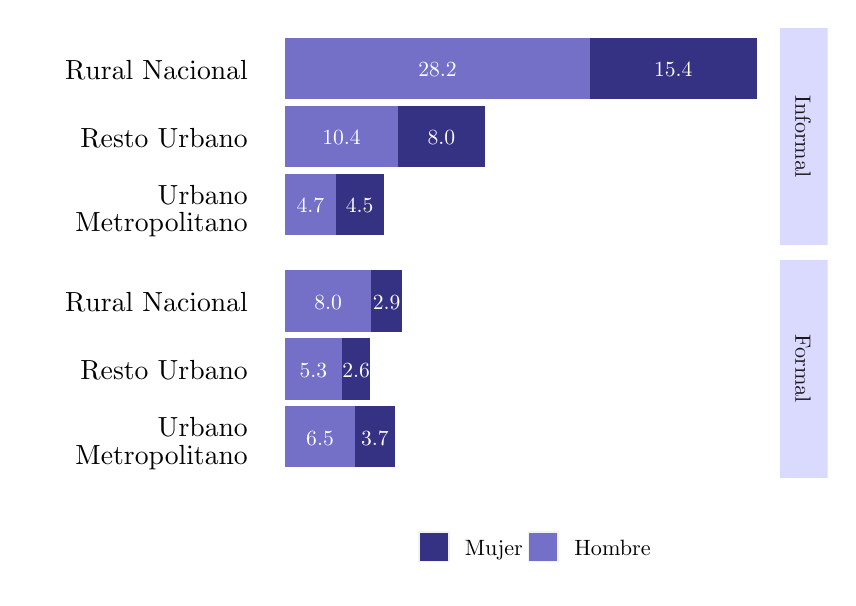
\begin{tikzpicture}[x=1pt,y=1pt]% Created by tikzDevice version 0.12.4 on 2023-05-04 16:38:58
% !TEX encoding = UTF-8 Unicode
\definecolor{fillColor}{RGB}{255,255,255}
\path[use as bounding box,fill=fillColor,fill opacity=0.00] (0,0) rectangle (289.08,198.74);
\begin{scope}
\path[clip] (  0.00,  0.00) rectangle (289.08,198.74);

\path[] (  0.00,  0.00) rectangle (289.08,198.74);
\end{scope}
\begin{scope}
\path[clip] (  0.00,  0.00) rectangle (289.08,198.74);
\definecolor{fillColor}{RGB}{54,50,131}

\path[fill=fillColor] (111.25,123.87) rectangle (128.68,145.96);
\definecolor{fillColor}{RGB}{116,112,200}

\path[fill=fillColor] ( 93.00,123.87) rectangle (111.25,145.96);
\definecolor{fillColor}{RGB}{54,50,131}

\path[fill=fillColor] (133.78,148.42) rectangle (165.15,170.51);
\definecolor{fillColor}{RGB}{116,112,200}

\path[fill=fillColor] ( 93.00,148.42) rectangle (133.78,170.51);
\definecolor{fillColor}{RGB}{54,50,131}

\path[fill=fillColor] (203.14,172.97) rectangle (263.40,195.06);
\definecolor{fillColor}{RGB}{116,112,200}

\path[fill=fillColor] ( 93.00,172.97) rectangle (203.14,195.06);
\definecolor{drawColor}{RGB}{255,255,255}

\node[text=drawColor,anchor=base,inner sep=0pt, outer sep=0pt, scale=  0.78] at (119.96,131.88) {4.5};

\node[text=drawColor,anchor=base,inner sep=0pt, outer sep=0pt, scale=  0.78] at (102.13,131.88) {4.7};

\node[text=drawColor,anchor=base,inner sep=0pt, outer sep=0pt, scale=  0.78] at (149.46,156.43) {8.0};

\node[text=drawColor,anchor=base,inner sep=0pt, outer sep=0pt, scale=  0.78] at (113.39,156.43) {10.4};

\node[text=drawColor,anchor=base,inner sep=0pt, outer sep=0pt, scale=  0.78] at (233.27,180.98) {15.4};

\node[text=drawColor,anchor=base,inner sep=0pt, outer sep=0pt, scale=  0.78] at (148.07,180.98) {28.2};

\path[] ( 84.48,134.92) --
	(271.92,134.92);

\path[] ( 84.48,159.46) --
	(271.92,159.46);

\path[] ( 84.48,184.01) --
	(271.92,184.01);

\path[] ( 84.48,120.19) rectangle (271.92,198.74);
\end{scope}
\begin{scope}
\path[clip] (  0.00,  0.00) rectangle (289.08,198.74);
\definecolor{fillColor}{RGB}{54,50,131}

\path[fill=fillColor] (118.27, 39.81) rectangle (132.74, 61.91);
\definecolor{fillColor}{RGB}{116,112,200}

\path[fill=fillColor] ( 93.00, 39.81) rectangle (118.27, 61.91);
\definecolor{fillColor}{RGB}{54,50,131}

\path[fill=fillColor] (113.55, 64.36) rectangle (123.85, 86.46);
\definecolor{fillColor}{RGB}{116,112,200}

\path[fill=fillColor] ( 93.00, 64.36) rectangle (113.55, 86.46);
\definecolor{fillColor}{RGB}{54,50,131}

\path[fill=fillColor] (124.12, 88.91) rectangle (135.38,111.00);
\definecolor{fillColor}{RGB}{116,112,200}

\path[fill=fillColor] ( 93.00, 88.91) rectangle (124.12,111.00);
\definecolor{drawColor}{RGB}{255,255,255}

\node[text=drawColor,anchor=base,inner sep=0pt, outer sep=0pt, scale=  0.78] at (125.50, 47.83) {3.7};

\node[text=drawColor,anchor=base,inner sep=0pt, outer sep=0pt, scale=  0.78] at (105.64, 47.83) {6.5};

\node[text=drawColor,anchor=base,inner sep=0pt, outer sep=0pt, scale=  0.78] at (118.70, 72.38) {2.6};

\node[text=drawColor,anchor=base,inner sep=0pt, outer sep=0pt, scale=  0.78] at (103.27, 72.38) {5.3};

\node[text=drawColor,anchor=base,inner sep=0pt, outer sep=0pt, scale=  0.78] at (129.75, 96.92) {2.9};

\node[text=drawColor,anchor=base,inner sep=0pt, outer sep=0pt, scale=  0.78] at (108.56, 96.92) {8.0};

\path[] ( 84.48, 50.86) --
	(271.92, 50.86);

\path[] ( 84.48, 75.41) --
	(271.92, 75.41);

\path[] ( 84.48, 99.96) --
	(271.92, 99.96);

\path[] ( 84.48, 36.13) rectangle (271.92,114.69);
\end{scope}
\begin{scope}
\path[clip] (  0.00,  0.00) rectangle (289.08,198.74);
\definecolor{fillColor}{RGB}{218,217,255}

\path[fill=fillColor] (271.92,120.19) rectangle (289.08,198.74);
\definecolor{drawColor}{gray}{0.10}

\node[text=drawColor,rotate=-90.00,anchor=base,inner sep=0pt, outer sep=0pt, scale=  0.80] at (277.37,159.46) {Informal};
\end{scope}
\begin{scope}
\path[clip] (  0.00,  0.00) rectangle (289.08,198.74);
\definecolor{fillColor}{RGB}{218,217,255}

\path[fill=fillColor] (271.92, 36.13) rectangle (289.08,114.69);
\definecolor{drawColor}{gray}{0.10}

\node[text=drawColor,rotate=-90.00,anchor=base,inner sep=0pt, outer sep=0pt, scale=  0.80] at (277.37, 75.41) {Formal};
\end{scope}
\begin{scope}
\path[clip] (  0.00,  0.00) rectangle (289.08,198.74);

\path[] ( 84.48, 36.13) --
	(271.92, 36.13);
\end{scope}
\begin{scope}
\path[clip] (  0.00,  0.00) rectangle (289.08,198.74);

\path[] ( 93.00, 33.38) --
	( 93.00, 36.13);

\path[] (132.12, 33.38) --
	(132.12, 36.13);

\path[] (171.24, 33.38) --
	(171.24, 36.13);

\path[] (210.36, 33.38) --
	(210.36, 36.13);

\path[] (249.48, 33.38) --
	(249.48, 36.13);
\end{scope}
\begin{scope}
\path[clip] (  0.00,  0.00) rectangle (289.08,198.74);

\path[] ( 84.48,120.19) --
	( 84.48,198.74);
\end{scope}
\begin{scope}
\path[clip] (  0.00,  0.00) rectangle (289.08,198.74);
\definecolor{drawColor}{RGB}{0,0,0}

\node[text=drawColor,anchor=base east,inner sep=0pt, outer sep=0pt, scale=  1.00] at ( 79.53,135.01) {Urbano};

\node[text=drawColor,anchor=base east,inner sep=0pt, outer sep=0pt, scale=  1.00] at ( 79.53,125.01) {Metropolitano};

\node[text=drawColor,anchor=base east,inner sep=0pt, outer sep=0pt, scale=  1.00] at ( 79.53,155.56) {Resto Urbano};

\node[text=drawColor,anchor=base east,inner sep=0pt, outer sep=0pt, scale=  1.00] at ( 79.53,180.10) {Rural Nacional};
\end{scope}
\begin{scope}
\path[clip] (  0.00,  0.00) rectangle (289.08,198.74);

\path[] ( 81.73,134.92) --
	( 84.48,134.92);

\path[] ( 81.73,159.46) --
	( 84.48,159.46);

\path[] ( 81.73,184.01) --
	( 84.48,184.01);
\end{scope}
\begin{scope}
\path[clip] (  0.00,  0.00) rectangle (289.08,198.74);

\path[] ( 84.48, 36.13) --
	( 84.48,114.69);
\end{scope}
\begin{scope}
\path[clip] (  0.00,  0.00) rectangle (289.08,198.74);
\definecolor{drawColor}{RGB}{0,0,0}

\node[text=drawColor,anchor=base east,inner sep=0pt, outer sep=0pt, scale=  1.00] at ( 79.53, 50.95) {Urbano};

\node[text=drawColor,anchor=base east,inner sep=0pt, outer sep=0pt, scale=  1.00] at ( 79.53, 40.95) {Metropolitano};

\node[text=drawColor,anchor=base east,inner sep=0pt, outer sep=0pt, scale=  1.00] at ( 79.53, 71.50) {Resto Urbano};

\node[text=drawColor,anchor=base east,inner sep=0pt, outer sep=0pt, scale=  1.00] at ( 79.53, 96.05) {Rural Nacional};
\end{scope}
\begin{scope}
\path[clip] (  0.00,  0.00) rectangle (289.08,198.74);

\path[] ( 81.73, 50.86) --
	( 84.48, 50.86);

\path[] ( 81.73, 75.41) --
	( 84.48, 75.41);

\path[] ( 81.73, 99.96) --
	( 84.48, 99.96);
\end{scope}
\begin{scope}
\path[clip] (  0.00,  0.00) rectangle (289.08,198.74);
\definecolor{fillColor}{RGB}{255,255,255}

\path[fill=fillColor] (130.12, -0.00) rectangle (226.29, 22.38);
\end{scope}
\begin{scope}
\path[clip] (  0.00,  0.00) rectangle (289.08,198.74);
\definecolor{fillColor}{gray}{0.95}

\path[fill=fillColor] (141.12,  5.50) rectangle (152.50, 16.88);
\end{scope}
\begin{scope}
\path[clip] (  0.00,  0.00) rectangle (289.08,198.74);
\definecolor{fillColor}{RGB}{54,50,131}

\path[fill=fillColor] (141.78,  6.16) rectangle (151.84, 16.22);
\end{scope}
\begin{scope}
\path[clip] (  0.00,  0.00) rectangle (289.08,198.74);
\definecolor{fillColor}{gray}{0.95}

\path[fill=fillColor] (180.66,  5.50) rectangle (192.04, 16.88);
\end{scope}
\begin{scope}
\path[clip] (  0.00,  0.00) rectangle (289.08,198.74);
\definecolor{fillColor}{RGB}{116,112,200}

\path[fill=fillColor] (181.32,  6.16) rectangle (191.38, 16.22);
\end{scope}
\begin{scope}
\path[clip] (  0.00,  0.00) rectangle (289.08,198.74);
\definecolor{drawColor}{RGB}{0,0,0}

\node[text=drawColor,anchor=base west,inner sep=0pt, outer sep=0pt, scale=  0.80] at (158.00,  8.06) {Mujer};
\end{scope}
\begin{scope}
\path[clip] (  0.00,  0.00) rectangle (289.08,198.74);
\definecolor{drawColor}{RGB}{0,0,0}

\node[text=drawColor,anchor=base west,inner sep=0pt, outer sep=0pt, scale=  0.80] at (197.54,  8.06) {Hombre};
\end{scope}
\end{tikzpicture}}{INE - ENEI 2022}{}

\cajita{Población ocupada por sexo, según rango de edad}{Se define a la Población Ocupada (PO) como las personas mayores de 15 años o más que realizaron algún tipo de actividad económica durante la semana. 

Para 2022, las mujeres que integraron la PO en las edades de 15 a 29 años representaron el 12.5\% del total de la PO, aquellas entre 30 y 65 años representaron el 22.7\% y de las mujeres de 65 años en adelante representa el 1.9\%.}{PEA por sexo, según dominio de estudio Y sector económico}{República de Guatemala, Instituto Nacional de Estadística -INE- en porcentaje} {\begin{tikzpicture}[x=1pt,y=1pt]% Created by tikzDevice version 0.12.4 on 2023-04-26 13:51:39
% !TEX encoding = UTF-8 Unicode
\definecolor{fillColor}{RGB}{255,255,255}
\path[use as bounding box,fill=fillColor,fill opacity=0.00] (0,0) rectangle (289.08,198.74);
\begin{scope}
\path[clip] (  0.00,  0.00) rectangle (289.08,198.74);

\path[] (  0.00,  0.00) rectangle (289.08,198.74);
\end{scope}
\begin{scope}
\path[clip] (  0.00,  0.00) rectangle (289.08,198.74);
\definecolor{fillColor}{RGB}{54,50,131}

\path[fill=fillColor] ( 15.81, 21.09) rectangle ( 51.94, 72.93);

\path[fill=fillColor] (106.15, 21.09) rectangle (142.28,114.98);

\path[fill=fillColor] (196.48, 21.09) rectangle (232.62, 28.83);
\definecolor{fillColor}{RGB}{116,112,200}

\path[fill=fillColor] ( 56.46, 21.09) rectangle ( 92.60,112.77);

\path[fill=fillColor] (146.80, 21.09) rectangle (182.93,170.58);

\path[fill=fillColor] (237.14, 21.09) rectangle (273.27, 40.24);
\definecolor{drawColor}{RGB}{0,0,0}

\path[draw=drawColor,line width= 0.6pt,line join=round] (-289.08, 21.09) -- (578.16, 21.09);

\node[text=drawColor,anchor=base,inner sep=0pt, outer sep=0pt, scale=  0.83] at ( 33.88, 76.17) {12.5};

\node[text=drawColor,anchor=base,inner sep=0pt, outer sep=0pt, scale=  0.83] at (124.21,118.21) {22.7};

\node[text=drawColor,anchor=base,inner sep=0pt, outer sep=0pt, scale=  0.83] at (214.55, 32.06) {1.9};

\node[text=drawColor,anchor=base,inner sep=0pt, outer sep=0pt, scale=  0.83] at ( 74.53,116.01) {22.2};

\node[text=drawColor,anchor=base,inner sep=0pt, outer sep=0pt, scale=  0.83] at (164.87,173.81) {36.1};

\node[text=drawColor,anchor=base,inner sep=0pt, outer sep=0pt, scale=  0.83] at (255.20, 43.48) {4.6};

\path[] (  0.00, 21.09) rectangle (289.08,170.58);

\path[] ( 54.20, 21.09) --
	( 54.20,170.58);

\path[] (144.54, 21.09) --
	(144.54,170.58);

\path[] (234.88, 21.09) --
	(234.88,170.58);

\path[] (  0.00, 21.09) rectangle (289.08,170.58);
\end{scope}
\begin{scope}
\path[clip] (  0.00,  0.00) rectangle (289.08,198.74);

\path[] (  0.00, 21.09) --
	(  0.00,170.58);
\end{scope}
\begin{scope}
\path[clip] (  0.00,  0.00) rectangle (289.08,198.74);

\path[] (  0.00, 21.09) --
	(289.08, 21.09);
\end{scope}
\begin{scope}
\path[clip] (  0.00,  0.00) rectangle (289.08,198.74);

\path[] ( 54.20, 18.34) --
	( 54.20, 21.09);

\path[] (144.54, 18.34) --
	(144.54, 21.09);

\path[] (234.88, 18.34) --
	(234.88, 21.09);
\end{scope}
\begin{scope}
\path[clip] (  0.00,  0.00) rectangle (289.08,198.74);
\definecolor{drawColor}{RGB}{0,0,0}

\node[text=drawColor,anchor=base,inner sep=0pt, outer sep=0pt, scale=  1.00] at ( 54.20,  7.01) {15-29};

\node[text=drawColor,anchor=base,inner sep=0pt, outer sep=0pt, scale=  1.00] at (144.54,  7.01) {30-65};

\node[text=drawColor,anchor=base,inner sep=0pt, outer sep=0pt, scale=  1.00] at (234.88,  7.01) {65+};
\end{scope}
\begin{scope}
\path[clip] (  0.00,  0.00) rectangle (289.08,198.74);
\coordinate (apoyo) at (59.42,189.21);
\coordinate (longitudFicticia) at (7.11,9.53);
\coordinate (longitud) at (7.11,7.11);
\coordinate (desX) at (135.34,0);
\coordinate (desY) at (0,1.21);
\definecolor[named]{ct1}{HTML}{
363283
}
\definecolor[named]{ct2}{HTML}{
7470C8
}
\definecolor[named]{ctb1}{HTML}{
363283
}
\definecolor[named]{ctb2}{HTML}{
7470C8
}
\path [fill=none] (apoyo) rectangle ($(apoyo)+(longitudFicticia)$)
node [xshift=0.3cm,inner sep=0pt, outer sep=0pt,midway,right,scale = 0.9]{Mujeres};
\draw [color = ctb1,fill=ct1] ( $(apoyo)  + (desY) $) rectangle ($(apoyo)+ (desY) +(longitud)$);
\path [fill=none] ($(apoyo)+(desX)$) rectangle ($(apoyo)+(desX)+(longitudFicticia)$)
node [xshift=0.3cm,inner sep=0pt, outer sep=0pt,midway,right,scale = 0.9]{Hombres};
\draw [color = ctb2 ,fill=ct2] ( $(apoyo)  + (desY) + (desX) $) rectangle ($(apoyo)+ (desY)+ (desX) +(longitud)$);
\end{scope}
\end{tikzpicture}}{INE - ENEI 2022}{}

\cajita{Población ocupada por sexo, según categoría ocupaciona}{Se muestra la categoría ocupacional de la Población Ocupada en Guatemala. A nivel nacional las tres categorías predominantes en las mujeres son trabajadoras por Cuenta propia no agrícola con el 12.4\%, seguido de Empleada de empresa privada con el 10.3\% y trabajadoras de Servicio doméstico con el 4.0\%.
}{Población ocupada por sexo, según dominio de estudio y categoría ocupaciona}{República de Guatemala, Instituto Nacional de Estadística -INE- en porcentaje} {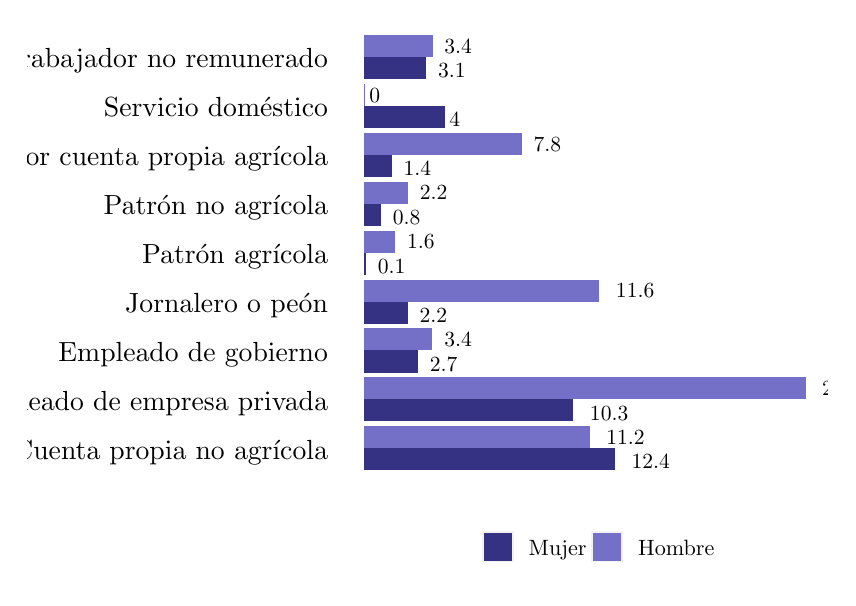
\begin{tikzpicture}[x=1pt,y=1pt]% Created by tikzDevice version 0.12.4 on 2023-05-05 16:55:51
% !TEX encoding = UTF-8 Unicode
\definecolor{fillColor}{RGB}{255,255,255}
\path[use as bounding box,fill=fillColor,fill opacity=0.00] (0,0) rectangle (289.08,198.74);
\begin{scope}
\path[clip] (  0.00,  0.00) rectangle (289.08,198.74);

\path[] (  0.00,  0.00) rectangle (289.08,198.74);
\end{scope}
\begin{scope}
\path[clip] (  0.00,  0.00) rectangle (289.08,198.74);
\definecolor{fillColor}{RGB}{54,50,131}

\path[fill=fillColor] (121.42, 74.13) rectangle (141.07, 82.09);

\path[fill=fillColor] (121.42, 56.46) rectangle (197.22, 64.41);

\path[fill=fillColor] (121.42, 91.81) rectangle (137.32, 99.76);

\path[fill=fillColor] (121.42,162.51) rectangle (150.69,170.46);

\path[fill=fillColor] (121.42, 38.78) rectangle (212.28, 46.74);

\path[fill=fillColor] (121.42,127.16) rectangle (127.64,135.11);

\path[fill=fillColor] (121.42,144.83) rectangle (131.59,152.79);

\path[fill=fillColor] (121.42,109.48) rectangle (122.23,117.44);

\path[fill=fillColor] (121.42,180.18) rectangle (144.01,188.14);
\definecolor{fillColor}{RGB}{116,112,200}

\path[fill=fillColor] (121.42, 82.09) rectangle (146.28, 90.04);

\path[fill=fillColor] (121.42, 64.41) rectangle (281.10, 72.37);

\path[fill=fillColor] (121.42, 99.76) rectangle (206.62,107.72);

\path[fill=fillColor] (121.42,170.46) rectangle (121.75,178.42);

\path[fill=fillColor] (121.42, 46.74) rectangle (203.12, 54.69);

\path[fill=fillColor] (121.42,135.11) rectangle (137.42,143.07);

\path[fill=fillColor] (121.42,152.79) rectangle (178.51,160.74);

\path[fill=fillColor] (121.42,117.44) rectangle (132.83,125.39);

\path[fill=fillColor] (121.42,188.14) rectangle (146.31,196.09);
\definecolor{drawColor}{RGB}{0,0,0}

\node[text=drawColor,anchor=base west,inner sep=0pt, outer sep=0pt, scale=  0.78] at (145.35, 74.63) {2.7};

\node[text=drawColor,anchor=base west,inner sep=0pt, outer sep=0pt, scale=  0.78] at (203.19, 56.96) {10.3};

\node[text=drawColor,anchor=base west,inner sep=0pt, outer sep=0pt, scale=  0.78] at (141.59, 92.31) {2.2};

\node[text=drawColor,anchor=base west,inner sep=0pt, outer sep=0pt, scale=  0.78] at (152.39,163.01) {4};

\node[text=drawColor,anchor=base west,inner sep=0pt, outer sep=0pt, scale=  0.78] at (218.25, 39.28) {12.4};

\node[text=drawColor,anchor=base west,inner sep=0pt, outer sep=0pt, scale=  0.78] at (131.92,127.66) {0.8};

\node[text=drawColor,anchor=base west,inner sep=0pt, outer sep=0pt, scale=  0.78] at (135.87,145.34) {1.4};

\node[text=drawColor,anchor=base west,inner sep=0pt, outer sep=0pt, scale=  0.78] at (126.50,109.99) {0.1};

\node[text=drawColor,anchor=base west,inner sep=0pt, outer sep=0pt, scale=  0.78] at (148.28,180.69) {3.1};

\node[text=drawColor,anchor=base west,inner sep=0pt, outer sep=0pt, scale=  0.78] at (150.56, 83.47) {3.4};

\node[text=drawColor,anchor=base west,inner sep=0pt, outer sep=0pt, scale=  0.78] at (287.07, 65.80) {21.8};

\node[text=drawColor,anchor=base west,inner sep=0pt, outer sep=0pt, scale=  0.78] at (212.59,101.15) {11.6};

\node[text=drawColor,anchor=base west,inner sep=0pt, outer sep=0pt, scale=  0.78] at (123.45,171.85) {0};

\node[text=drawColor,anchor=base west,inner sep=0pt, outer sep=0pt, scale=  0.78] at (209.09, 48.12) {11.2};

\node[text=drawColor,anchor=base west,inner sep=0pt, outer sep=0pt, scale=  0.78] at (141.70,136.50) {2.2};

\node[text=drawColor,anchor=base west,inner sep=0pt, outer sep=0pt, scale=  0.78] at (182.79,154.17) {7.8};

\node[text=drawColor,anchor=base west,inner sep=0pt, outer sep=0pt, scale=  0.78] at (137.10,118.82) {1.6};

\node[text=drawColor,anchor=base west,inner sep=0pt, outer sep=0pt, scale=  0.78] at (150.59,189.52) {3.4};

\path[] (113.44, 46.74) --
	(289.08, 46.74);

\path[] (113.44, 64.41) --
	(289.08, 64.41);

\path[] (113.44, 82.09) --
	(289.08, 82.09);

\path[] (113.44, 99.76) --
	(289.08, 99.76);

\path[] (113.44,117.44) --
	(289.08,117.44);

\path[] (113.44,135.11) --
	(289.08,135.11);

\path[] (113.44,152.79) --
	(289.08,152.79);

\path[] (113.44,170.46) --
	(289.08,170.46);

\path[] (113.44,188.14) --
	(289.08,188.14);

\path[] (113.44, 36.13) rectangle (289.08,198.74);
\end{scope}
\begin{scope}
\path[clip] (  0.00,  0.00) rectangle (289.08,198.74);

\path[] (113.44, 36.13) --
	(113.44,198.74);
\end{scope}
\begin{scope}
\path[clip] (  0.00,  0.00) rectangle (289.08,198.74);
\definecolor{drawColor}{RGB}{0,0,0}

\node[text=drawColor,anchor=base east,inner sep=0pt, outer sep=0pt, scale=  1.00] at (108.49, 42.83) {Cuenta propia no agrícola};

\node[text=drawColor,anchor=base east,inner sep=0pt, outer sep=0pt, scale=  1.00] at (108.49, 60.50) {Empleado de empresa privada};

\node[text=drawColor,anchor=base east,inner sep=0pt, outer sep=0pt, scale=  1.00] at (108.49, 78.18) {Empleado de gobierno};

\node[text=drawColor,anchor=base east,inner sep=0pt, outer sep=0pt, scale=  1.00] at (108.49, 95.85) {Jornalero o peón};

\node[text=drawColor,anchor=base east,inner sep=0pt, outer sep=0pt, scale=  1.00] at (108.49,113.53) {Patrón agrícola};

\node[text=drawColor,anchor=base east,inner sep=0pt, outer sep=0pt, scale=  1.00] at (108.49,131.20) {Patrón no agrícola};

\node[text=drawColor,anchor=base east,inner sep=0pt, outer sep=0pt, scale=  1.00] at (108.49,148.88) {Por cuenta propia agrícola};

\node[text=drawColor,anchor=base east,inner sep=0pt, outer sep=0pt, scale=  1.00] at (108.49,166.55) {Servicio doméstico};

\node[text=drawColor,anchor=base east,inner sep=0pt, outer sep=0pt, scale=  1.00] at (108.49,184.23) {Trabajador no remunerado};
\end{scope}
\begin{scope}
\path[clip] (  0.00,  0.00) rectangle (289.08,198.74);

\path[] (110.69, 46.74) --
	(113.44, 46.74);

\path[] (110.69, 64.41) --
	(113.44, 64.41);

\path[] (110.69, 82.09) --
	(113.44, 82.09);

\path[] (110.69, 99.76) --
	(113.44, 99.76);

\path[] (110.69,117.44) --
	(113.44,117.44);

\path[] (110.69,135.11) --
	(113.44,135.11);

\path[] (110.69,152.79) --
	(113.44,152.79);

\path[] (110.69,170.46) --
	(113.44,170.46);

\path[] (110.69,188.14) --
	(113.44,188.14);
\end{scope}
\begin{scope}
\path[clip] (  0.00,  0.00) rectangle (289.08,198.74);

\path[] (113.44, 36.13) --
	(289.08, 36.13);
\end{scope}
\begin{scope}
\path[clip] (  0.00,  0.00) rectangle (289.08,198.74);

\path[] (121.42, 33.38) --
	(121.42, 36.13);

\path[] (158.04, 33.38) --
	(158.04, 36.13);

\path[] (194.66, 33.38) --
	(194.66, 36.13);

\path[] (231.28, 33.38) --
	(231.28, 36.13);

\path[] (267.90, 33.38) --
	(267.90, 36.13);
\end{scope}
\begin{scope}
\path[clip] (  0.00,  0.00) rectangle (289.08,198.74);
\definecolor{fillColor}{RGB}{255,255,255}

\path[fill=fillColor] (153.18, -0.00) rectangle (249.34, 22.38);
\end{scope}
\begin{scope}
\path[clip] (  0.00,  0.00) rectangle (289.08,198.74);
\definecolor{fillColor}{gray}{0.95}

\path[fill=fillColor] (164.18,  5.50) rectangle (175.56, 16.88);
\end{scope}
\begin{scope}
\path[clip] (  0.00,  0.00) rectangle (289.08,198.74);
\definecolor{fillColor}{RGB}{54,50,131}

\path[fill=fillColor] (164.84,  6.16) rectangle (174.90, 16.22);
\end{scope}
\begin{scope}
\path[clip] (  0.00,  0.00) rectangle (289.08,198.74);
\definecolor{fillColor}{gray}{0.95}

\path[fill=fillColor] (203.72,  5.50) rectangle (215.10, 16.88);
\end{scope}
\begin{scope}
\path[clip] (  0.00,  0.00) rectangle (289.08,198.74);
\definecolor{fillColor}{RGB}{116,112,200}

\path[fill=fillColor] (204.38,  6.16) rectangle (214.44, 16.22);
\end{scope}
\begin{scope}
\path[clip] (  0.00,  0.00) rectangle (289.08,198.74);
\definecolor{drawColor}{RGB}{0,0,0}

\node[text=drawColor,anchor=base west,inner sep=0pt, outer sep=0pt, scale=  0.80] at (181.06,  8.06) {Mujer};
\end{scope}
\begin{scope}
\path[clip] (  0.00,  0.00) rectangle (289.08,198.74);
\definecolor{drawColor}{RGB}{0,0,0}

\node[text=drawColor,anchor=base west,inner sep=0pt, outer sep=0pt, scale=  0.80] at (220.60,  8.06) {Hombre};
\end{scope}
\end{tikzpicture}}{INE - ENEI 2022}{}

\cajita{Población ocupada con acceso a seguro social por sexo, según actividad económica}{A nivel nacional, para 2022, las tres actividades económicas predominantes en mujeres que integraron la población ocupada que cuenta con acceso a seguro social fueron actividades de comercio con el 12.9\%, seguida de otras actividades de servicios con el 7.5\% y actividades de industria manufacturera con el 6.7\%. \footnote{Los resultados reportados no suman el cien por ciento y algunos dan 0.0\% debido al redondeo de los mismos.}}{Población ocupada con acceso a seguro social por sexo, según rama de actividad económica }{República de Guatemala, Instituto Nacional de Estadística -INE- en porcentaje} {\begin{tikzpicture}[x=1pt,y=1pt]% Created by tikzDevice version 0.12.4 on 2023-04-28 11:09:07
% !TEX encoding = UTF-8 Unicode
\definecolor{fillColor}{RGB}{255,255,255}
\path[use as bounding box,fill=fillColor,fill opacity=0.00] (0,0) rectangle (289.08,198.74);
\begin{scope}
\path[clip] (  0.00,  0.00) rectangle (289.08,198.74);

\path[] (  0.00,  0.00) rectangle (289.08,198.74);
\end{scope}
\begin{scope}
\path[clip] (  0.00,  0.00) rectangle (289.08,198.74);
\definecolor{fillColor}{RGB}{54,50,131}

\path[fill=fillColor] (  4.52, 21.09) rectangle ( 14.84, 44.81);

\path[fill=fillColor] ( 30.33, 21.09) rectangle ( 40.65, 63.77);

\path[fill=fillColor] ( 56.14, 21.09) rectangle ( 66.46, 21.39);

\path[fill=fillColor] ( 81.95, 21.09) rectangle ( 92.27,103.60);

\path[fill=fillColor] (107.76, 21.09) rectangle (118.08, 21.76);

\path[fill=fillColor] (133.57, 21.09) rectangle (143.89, 24.60);

\path[fill=fillColor] (159.38, 21.09) rectangle (169.71, 22.11);

\path[fill=fillColor] (185.19, 21.09) rectangle (195.52, 29.05);

\path[fill=fillColor] (211.00, 21.09) rectangle (221.33, 47.03);

\path[fill=fillColor] (236.81, 21.09) rectangle (247.14, 69.11);

\path[fill=fillColor] (262.62, 21.09) rectangle (272.95, 21.92);
\definecolor{fillColor}{RGB}{116,112,200}

\path[fill=fillColor] ( 16.13, 21.09) rectangle ( 26.46,170.58);

\path[fill=fillColor] ( 41.94, 21.09) rectangle ( 52.27, 70.97);

\path[fill=fillColor] ( 67.75, 21.09) rectangle ( 78.08, 68.70);

\path[fill=fillColor] ( 93.56, 21.09) rectangle (103.89,112.19);

\path[fill=fillColor] (119.37, 21.09) rectangle (129.70, 24.16);

\path[fill=fillColor] (145.19, 21.09) rectangle (155.51, 25.70);

\path[fill=fillColor] (171.00, 21.09) rectangle (181.32, 22.23);

\path[fill=fillColor] (196.81, 21.09) rectangle (207.13, 36.99);

\path[fill=fillColor] (222.62, 21.09) rectangle (232.94, 45.65);

\path[fill=fillColor] (248.43, 21.09) rectangle (258.75, 35.53);

\path[fill=fillColor] (274.24, 21.09) rectangle (284.56, 21.59);
\definecolor{drawColor}{RGB}{0,0,0}

\path[draw=drawColor,line width= 0.6pt,line join=round] (-289.08, 21.09) -- (578.16, 21.09);

\node[text=drawColor,anchor=base,inner sep=0pt, outer sep=0pt, scale=  0.83] at (  9.68, 48.05) {3.7};

\node[text=drawColor,anchor=base,inner sep=0pt, outer sep=0pt, scale=  0.83] at ( 35.49, 67.01) {6.7};

\node[text=drawColor,anchor=base,inner sep=0pt, outer sep=0pt, scale=  0.83] at ( 61.30, 24.62) {0.0};

\node[text=drawColor,anchor=base,inner sep=0pt, outer sep=0pt, scale=  0.83] at ( 87.11,106.84) {12.9};

\node[text=drawColor,anchor=base,inner sep=0pt, outer sep=0pt, scale=  0.83] at (112.92, 25.00) {0.1};

\node[text=drawColor,anchor=base,inner sep=0pt, outer sep=0pt, scale=  0.83] at (138.73, 27.84) {0.5};

\node[text=drawColor,anchor=base,inner sep=0pt, outer sep=0pt, scale=  0.83] at (164.54, 25.35) {0.2};

\node[text=drawColor,anchor=base,inner sep=0pt, outer sep=0pt, scale=  0.83] at (190.35, 32.28) {1.2};

\node[text=drawColor,anchor=base,inner sep=0pt, outer sep=0pt, scale=  0.83] at (216.16, 50.26) {4.1};

\node[text=drawColor,anchor=base,inner sep=0pt, outer sep=0pt, scale=  0.83] at (241.98, 72.35) {7.5};

\node[text=drawColor,anchor=base,inner sep=0pt, outer sep=0pt, scale=  0.83] at (267.79, 25.15) {0.1};

\node[text=drawColor,anchor=base,inner sep=0pt, outer sep=0pt, scale=  0.83] at ( 21.29,173.81) {23.4};

\node[text=drawColor,anchor=base,inner sep=0pt, outer sep=0pt, scale=  0.83] at ( 47.10, 74.21) {7.8};

\node[text=drawColor,anchor=base,inner sep=0pt, outer sep=0pt, scale=  0.83] at ( 72.92, 71.94) {7.4};

\node[text=drawColor,anchor=base,inner sep=0pt, outer sep=0pt, scale=  0.83] at ( 98.73,115.43) {14.2};

\node[text=drawColor,anchor=base,inner sep=0pt, outer sep=0pt, scale=  0.83] at (124.54, 27.40) {0.5};

\node[text=drawColor,anchor=base,inner sep=0pt, outer sep=0pt, scale=  0.83] at (150.35, 28.94) {0.7};

\node[text=drawColor,anchor=base,inner sep=0pt, outer sep=0pt, scale=  0.83] at (176.16, 25.47) {0.2};

\node[text=drawColor,anchor=base,inner sep=0pt, outer sep=0pt, scale=  0.83] at (201.97, 40.23) {2.5};

\node[text=drawColor,anchor=base,inner sep=0pt, outer sep=0pt, scale=  0.83] at (227.78, 48.89) {3.8};

\node[text=drawColor,anchor=base,inner sep=0pt, outer sep=0pt, scale=  0.83] at (253.59, 38.76) {2.3};

\node[text=drawColor,anchor=base,inner sep=0pt, outer sep=0pt, scale=  0.83] at (279.40, 24.83) {0.1};

\path[] (  0.00, 21.09) rectangle (289.08,170.58);

\path[] ( 15.49, 21.09) --
	( 15.49,170.58);

\path[] ( 41.30, 21.09) --
	( 41.30,170.58);

\path[] ( 67.11, 21.09) --
	( 67.11,170.58);

\path[] ( 92.92, 21.09) --
	( 92.92,170.58);

\path[] (118.73, 21.09) --
	(118.73,170.58);

\path[] (144.54, 21.09) --
	(144.54,170.58);

\path[] (170.35, 21.09) --
	(170.35,170.58);

\path[] (196.16, 21.09) --
	(196.16,170.58);

\path[] (221.97, 21.09) --
	(221.97,170.58);

\path[] (247.78, 21.09) --
	(247.78,170.58);

\path[] (273.59, 21.09) --
	(273.59,170.58);

\path[] (  0.00, 21.09) rectangle (289.08,170.58);
\end{scope}
\begin{scope}
\path[clip] (  0.00,  0.00) rectangle (289.08,198.74);

\path[] (  0.00, 21.09) --
	(  0.00,170.58);
\end{scope}
\begin{scope}
\path[clip] (  0.00,  0.00) rectangle (289.08,198.74);

\path[] (  0.00, 21.09) --
	(289.08, 21.09);
\end{scope}
\begin{scope}
\path[clip] (  0.00,  0.00) rectangle (289.08,198.74);

\path[] ( 15.49, 18.34) --
	( 15.49, 21.09);

\path[] ( 41.30, 18.34) --
	( 41.30, 21.09);

\path[] ( 67.11, 18.34) --
	( 67.11, 21.09);

\path[] ( 92.92, 18.34) --
	( 92.92, 21.09);

\path[] (118.73, 18.34) --
	(118.73, 21.09);

\path[] (144.54, 18.34) --
	(144.54, 21.09);

\path[] (170.35, 18.34) --
	(170.35, 21.09);

\path[] (196.16, 18.34) --
	(196.16, 21.09);

\path[] (221.97, 18.34) --
	(221.97, 21.09);

\path[] (247.78, 18.34) --
	(247.78, 21.09);

\path[] (273.59, 18.34) --
	(273.59, 21.09);
\end{scope}
\begin{scope}
\path[clip] (  0.00,  0.00) rectangle (289.08,198.74);
\definecolor{drawColor}{RGB}{0,0,0}

\node[text=drawColor,anchor=base,inner sep=0pt, outer sep=0pt, scale=  1.00] at ( 15.49,  7.01) {Agricultura};

\node[text=drawColor,anchor=base,inner sep=0pt, outer sep=0pt, scale=  1.00] at ( 41.30,  7.01) {Industrias manufactureras};

\node[text=drawColor,anchor=base,inner sep=0pt, outer sep=0pt, scale=  1.00] at ( 67.11,  7.01) {Construcción};

\node[text=drawColor,anchor=base,inner sep=0pt, outer sep=0pt, scale=  1.00] at ( 92.92,  7.01) {Comercio};

\node[text=drawColor,anchor=base,inner sep=0pt, outer sep=0pt, scale=  1.00] at (118.73,  7.01) {Comunicaciones};

\node[text=drawColor,anchor=base,inner sep=0pt, outer sep=0pt, scale=  1.00] at (144.54,  7.01) {Financieras y de seguros};

\node[text=drawColor,anchor=base,inner sep=0pt, outer sep=0pt, scale=  1.00] at (170.35,  7.01) {Inmobiliarias};

\node[text=drawColor,anchor=base,inner sep=0pt, outer sep=0pt, scale=  1.00] at (196.16,  7.01) {Profesionales};

\node[text=drawColor,anchor=base,inner sep=0pt, outer sep=0pt, scale=  1.00] at (221.97,  7.01) {Administración pública};

\node[text=drawColor,anchor=base,inner sep=0pt, outer sep=0pt, scale=  1.00] at (247.78,  7.01) {Otras de servicios};

\node[text=drawColor,anchor=base,inner sep=0pt, outer sep=0pt, scale=  1.00] at (273.59,  7.01) {NS/NR};
\end{scope}
\begin{scope}
\path[clip] (  0.00,  0.00) rectangle (289.08,198.74);
\coordinate (apoyo) at (59.42,189.21);
\coordinate (longitudFicticia) at (7.11,9.53);
\coordinate (longitud) at (7.11,7.11);
\coordinate (desX) at (135.34,0);
\coordinate (desY) at (0,1.21);
\definecolor[named]{ct1}{HTML}{
363283
}
\definecolor[named]{ct2}{HTML}{
7470C8
}
\definecolor[named]{ctb1}{HTML}{
363283
}
\definecolor[named]{ctb2}{HTML}{
7470C8
}
\path [fill=none] (apoyo) rectangle ($(apoyo)+(longitudFicticia)$)
node [xshift=0.3cm,inner sep=0pt, outer sep=0pt,midway,right,scale = 0.9]{Mujer};
\draw [color = ctb1,fill=ct1] ( $(apoyo)  + (desY) $) rectangle ($(apoyo)+ (desY) +(longitud)$);
\path [fill=none] ($(apoyo)+(desX)$) rectangle ($(apoyo)+(desX)+(longitudFicticia)$)
node [xshift=0.3cm,inner sep=0pt, outer sep=0pt,midway,right,scale = 0.9]{Hombre};
\draw [color = ctb2 ,fill=ct2] ( $(apoyo)  + (desY) + (desX) $) rectangle ($(apoyo)+ (desY)+ (desX) +(longitud)$);
\end{scope}
\end{tikzpicture}}{INE - ENEI 2022}{}

\cajita{Créditos otorgados a la pequeña y mediana empresa por sexo (comparar 2018 y 2022)}{Según los Registros de la Unidad Financiera Programa Nacional para el Desarrollo de la MIPYME del Ministerio de Economía, se entregaron 766 créditos en 2022, a diferencia de 2018 que se entregaron 1,000 créditos a mujeres.

En 2018 la diferencia entre créditos otorgados a hombres y mujeres fue de 288 créditos. Para 2022 la diferencia fue de 291 créditos entre hombres y mujeres. }{Créditos otorgados a la pequeña y mediana empresa por sexo}{República de Guatemala, Instituto Nacional de Estadística -INE- en Número de Créditos} {\begin{tikzpicture}[x=1pt,y=1pt]% Created by tikzDevice version 0.12.4 on 2023-05-02 11:58:10
% !TEX encoding = UTF-8 Unicode
\definecolor{fillColor}{RGB}{255,255,255}
\path[use as bounding box,fill=fillColor,fill opacity=0.00] (0,0) rectangle (289.08,198.74);
\begin{scope}
\path[clip] (  0.00,  0.00) rectangle (289.08,198.74);

\path[] (  0.00,  0.00) rectangle (289.08,198.74);
\end{scope}
\begin{scope}
\path[clip] (  0.00,  0.00) rectangle (289.08,198.74);
\definecolor{fillColor}{RGB}{54,50,131}

\path[fill=fillColor] ( 23.00, 21.09) rectangle ( 75.55,137.15);

\path[fill=fillColor] (154.39, 21.09) rectangle (206.95,109.99);
\definecolor{fillColor}{RGB}{116,112,200}

\path[fill=fillColor] ( 82.13, 21.09) rectangle (134.68,170.58);

\path[fill=fillColor] (213.53, 21.09) rectangle (266.08,143.77);
\definecolor{drawColor}{RGB}{0,0,0}

\path[draw=drawColor,line width= 0.6pt,line join=round] (-289.08, 21.09) -- (578.16, 21.09);

\node[text=drawColor,anchor=base,inner sep=0pt, outer sep=0pt, scale=  0.83] at ( 49.27,140.39) {1,000};

\node[text=drawColor,anchor=base,inner sep=0pt, outer sep=0pt, scale=  0.83] at (180.68,113.23) {766};

\node[text=drawColor,anchor=base,inner sep=0pt, outer sep=0pt, scale=  0.83] at (108.41,173.81) {1,288};

\node[text=drawColor,anchor=base,inner sep=0pt, outer sep=0pt, scale=  0.83] at (239.81,147.00) {1,057};

\path[] (  0.00, 21.09) rectangle (289.08,170.58);

\path[] ( 78.84, 21.09) --
	( 78.84,170.58);

\path[] (210.24, 21.09) --
	(210.24,170.58);

\path[] (  0.00, 21.09) rectangle (289.08,170.58);
\end{scope}
\begin{scope}
\path[clip] (  0.00,  0.00) rectangle (289.08,198.74);

\path[] (  0.00, 21.09) --
	(  0.00,170.58);
\end{scope}
\begin{scope}
\path[clip] (  0.00,  0.00) rectangle (289.08,198.74);

\path[] (  0.00, 21.09) --
	(289.08, 21.09);
\end{scope}
\begin{scope}
\path[clip] (  0.00,  0.00) rectangle (289.08,198.74);

\path[] ( 78.84, 18.34) --
	( 78.84, 21.09);

\path[] (210.24, 18.34) --
	(210.24, 21.09);
\end{scope}
\begin{scope}
\path[clip] (  0.00,  0.00) rectangle (289.08,198.74);
\definecolor{drawColor}{RGB}{0,0,0}

\node[text=drawColor,anchor=base,inner sep=0pt, outer sep=0pt, scale=  1.00] at ( 78.84,  7.01) {2018};

\node[text=drawColor,anchor=base,inner sep=0pt, outer sep=0pt, scale=  1.00] at (210.24,  7.01) {2022};
\end{scope}
\begin{scope}
\path[clip] (  0.00,  0.00) rectangle (289.08,198.74);
\coordinate (apoyo) at (55.92,189.21);
\coordinate (longitudFicticia) at (7.11,9.53);
\coordinate (longitud) at (7.11,7.11);
\coordinate (desX) at (137.28,0);
\coordinate (desY) at (0,1.21);
\definecolor[named]{ct1}{HTML}{
363283
}
\definecolor[named]{ct2}{HTML}{
7470C8
}
\definecolor[named]{ctb1}{HTML}{
363283
}
\definecolor[named]{ctb2}{HTML}{
7470C8
}
\path [fill=none] (apoyo) rectangle ($(apoyo)+(longitudFicticia)$)
node [xshift=0.3cm,inner sep=0pt, outer sep=0pt,midway,right,scale = 0.9]{Mujeres};
\draw [color = ctb1,fill=ct1] ( $(apoyo)  + (desY) $) rectangle ($(apoyo)+ (desY) +(longitud)$);
\path [fill=none] ($(apoyo)+(desX)$) rectangle ($(apoyo)+(desX)+(longitudFicticia)$)
node [xshift=0.3cm,inner sep=0pt, outer sep=0pt,midway,right,scale = 0.9]{Hombres};
\draw [color = ctb2 ,fill=ct2] ( $(apoyo)  + (desY) + (desX) $) rectangle ($(apoyo)+ (desY)+ (desX) +(longitud)$);
\end{scope}
\end{tikzpicture}}{Registros Unidad Financiera Programa Nacional para el Desarrollo de la MIPYME, MINECO 2023}{}

\cajita{Créditos otorgados a la pequeña y mediana empresa por sexo, según rama de actividad económica (comparar 2018 y 2022)}{Según los Registros de la Unidad Financiera Programa Nacional para el Desarrollo de la MIPYME del Ministerio de Economía, las principales actividades económicas a las que se entregaron créditos a mujeres en 2022 fueron a Comercio con 640 créditos, seguido de Servicios con 91 créditos y Artesanías con 9 créditos. En 2018 se entregaron 865 créditos en Comercio, seguido de Servicios con 87 créditos e Industria con 31 créditos otorgados a mujeres. }{Créditos otorgados a la pequeña y mediana empresa por sexo, según rama de actividad económica}{República de Guatemala, Instituto Nacional de Estadística -INE-, en porcentaje}{\begin{tabular}[t]{ccccc}
\toprule
\multicolumn{1}{c}{\textbf{ }} & \multicolumn{2}{c}{\textbf{2018}} & \multicolumn{2}{c}{\textbf{2022}} \\
\cmidrule(l{3pt}r{3pt}){2-3} \cmidrule(l{3pt}r{3pt}){4-5}
\textbf{Actividad Económica} & \textbf{Mujeres} & \textbf{Hombres} & \textbf{Mujeres} & \textbf{Hombres}\\
\midrule
\cellcolor[HTML]{B6B3FF}{Comercio} & \cellcolor[HTML]{B6B3FF}{865} & \cellcolor[HTML]{B6B3FF}{1050} & \cellcolor[HTML]{B6B3FF}{640} & \cellcolor[HTML]{B6B3FF}{836}\\
Servicios & 87 & 155 & 91 & 159\\
\cellcolor[HTML]{B6B3FF}{Industria} & \cellcolor[HTML]{B6B3FF}{31} & \cellcolor[HTML]{B6B3FF}{52} & \cellcolor[HTML]{B6B3FF}{9} & \cellcolor[HTML]{B6B3FF}{30}\\
Artesanía & 12 & 26 & 15 & 18\\
\cellcolor[HTML]{B6B3FF}{Agroindustria} & \cellcolor[HTML]{B6B3FF}{5} & \cellcolor[HTML]{B6B3FF}{5} & \cellcolor[HTML]{B6B3FF}{11} & \cellcolor[HTML]{B6B3FF}{14}\\
\bottomrule
\end{tabular}
}{Registros Unidad Financiera Programa Nacional para el Desarrollo de la MIPYME, MINECO 2023}{}

%\cajota{Población por sexo, según grupos de edad}{El sector informal guatemalteco comprende a la Población Ocupada (PO) que labora como empleadores, empleados y obreros de empresas con menos de 6 personas, trabajadores por cuenta propia o autónoma (excluyendo profesionales y técnicos), familiares no remunerados de los empleadores o personas ocupadas en servicio doméstico. Su contraparte, el sector formal, está comprendido por la población ocupada que no está en el sector informal. 

En el año 2022 las mujeres integraron el 27.9\% del sector informal y el 9.2\% del sector formal. }{Población por sexo, según grupos de edad}{República de Guatemala, Instituto Nacional de Estadística -INE-, en miles de personas}{\begin{tikzpicture}[x=1pt,y=1pt, scale=1.75]% Created by tikzDevice version 0.12.4 on 2023-05-04 15:41:55
% !TEX encoding = UTF-8 Unicode
\definecolor{fillColor}{RGB}{255,255,255}
\path[use as bounding box,fill=fillColor,fill opacity=0.00] (0,0) rectangle (289.08,198.74);
\begin{scope}
\path[clip] (  0.00,  0.00) rectangle (289.08,198.74);

\path[] (  0.00,  0.00) rectangle (289.08,198.74);
\end{scope}
\begin{scope}
\path[clip] (  0.00,  0.00) rectangle (289.08,198.74);
\definecolor{fillColor}{RGB}{54,50,131}

\path[fill=fillColor] ( 23.00, 21.09) rectangle ( 75.55, 52.92);

\path[fill=fillColor] (154.39, 21.09) rectangle (206.95,117.47);
\definecolor{fillColor}{RGB}{116,112,200}

\path[fill=fillColor] ( 82.13, 21.09) rectangle (134.68, 89.08);

\path[fill=fillColor] (213.53, 21.09) rectangle (266.08,170.58);
\definecolor{drawColor}{RGB}{0,0,0}

\path[draw=drawColor,line width= 0.6pt,line join=round] (-289.08, 21.09) -- (578.16, 21.09);

\node[text=drawColor,anchor=base,inner sep=0pt, outer sep=0pt, scale=  0.83] at ( 49.27, 56.15) {9.2};

\node[text=drawColor,anchor=base,inner sep=0pt, outer sep=0pt, scale=  0.83] at (180.68,120.70) {27.9};

\node[text=drawColor,anchor=base,inner sep=0pt, outer sep=0pt, scale=  0.83] at (108.41, 92.31) {19.7};

\node[text=drawColor,anchor=base,inner sep=0pt, outer sep=0pt, scale=  0.83] at (239.81,173.81) {43.2};

\path[] (  0.00, 21.09) rectangle (289.08,170.58);

\path[] ( 78.84, 21.09) --
	( 78.84,170.58);

\path[] (210.24, 21.09) --
	(210.24,170.58);

\path[] (  0.00, 21.09) rectangle (289.08,170.58);
\end{scope}
\begin{scope}
\path[clip] (  0.00,  0.00) rectangle (289.08,198.74);

\path[] (  0.00, 21.09) --
	(  0.00,170.58);
\end{scope}
\begin{scope}
\path[clip] (  0.00,  0.00) rectangle (289.08,198.74);

\path[] (  0.00, 21.09) --
	(289.08, 21.09);
\end{scope}
\begin{scope}
\path[clip] (  0.00,  0.00) rectangle (289.08,198.74);

\path[] ( 78.84, 18.34) --
	( 78.84, 21.09);

\path[] (210.24, 18.34) --
	(210.24, 21.09);
\end{scope}
\begin{scope}
\path[clip] (  0.00,  0.00) rectangle (289.08,198.74);
\definecolor{drawColor}{RGB}{0,0,0}

\node[text=drawColor,anchor=base,inner sep=0pt, outer sep=0pt, scale=  1.00] at ( 78.84,  7.01) {Formal};

\node[text=drawColor,anchor=base,inner sep=0pt, outer sep=0pt, scale=  1.00] at (210.24,  7.01) {infromal};
\end{scope}
\begin{scope}
\path[clip] (  0.00,  0.00) rectangle (289.08,198.74);
\coordinate (apoyo) at (59.42,189.21);
\coordinate (longitudFicticia) at (7.11,9.53);
\coordinate (longitud) at (7.11,7.11);
\coordinate (desX) at (135.34,0);
\coordinate (desY) at (0,1.21);
\definecolor[named]{ct1}{HTML}{
363283
}
\definecolor[named]{ct2}{HTML}{
7470C8
}
\definecolor[named]{ctb1}{HTML}{
363283
}
\definecolor[named]{ctb2}{HTML}{
7470C8
}
\path [fill=none] (apoyo) rectangle ($(apoyo)+(longitudFicticia)$)
node [xshift=0.3cm,inner sep=0pt, outer sep=0pt,midway,right,scale = 0.9]{Mujer};
\draw [color = ctb1,fill=ct1] ( $(apoyo)  + (desY) $) rectangle ($(apoyo)+ (desY) +(longitud)$);
\path [fill=none] ($(apoyo)+(desX)$) rectangle ($(apoyo)+(desX)+(longitudFicticia)$)
node [xshift=0.3cm,inner sep=0pt, outer sep=0pt,midway,right,scale = 0.9]{Hombre};
\draw [color = ctb2 ,fill=ct2] ( $(apoyo)  + (desY) + (desX) $) rectangle ($(apoyo)+ (desY)+ (desX) +(longitud)$);
\end{scope}
\end{tikzpicture}}{INE - Censo 2018}